\documentclass[accentcolor=tud1c,colorback,ngerman,12pt] {tudreport}
\usepackage[utf8]{inputenc}
\usepackage{babel}
\usepackage{acronym}
\usepackage{listings}
\usepackage{tabularx}
\usepackage{url}
\usepackage{hyperref}
\usepackage{tikz}
\usepackage{circuitikz}
\usepackage{placeins}

\lstset{numbers=left, numberstyle=\tiny, numbersep=5pt}
\lstset{language=Java}

\renewcommand{\lstlistingname}{Quelltext}
\lstset{literate=%
{Ö}{{\"O}}1
{Ä}{{\"A}}1
{Ü}{{\"U}}1
{ß}{{\ss}}1
{ü}{{\"u}}1
{ä}{{\"a}}1
{ö}{{\"o}}1
}

\setinstitutionlogo[height]{bilder/rechnersysteme-transparent}

\begin{document}
\title{Implementierung eines multithreaded TCP/IP Stacks für einen auf AMIDAR basierten Java Prozessor}
\subtitle{Bachelorarbeit}
\subsubtitle{Robert Wiesner \hfill  \\31. Mai 2017}

\maketitle
\chapter*{Erklärung gemäß § 22 Abs. 7 APB}

Hiermit erkläre ich gemäß § 22 Abs. 7 der Allgemeinen Prüfungsbestimmungen (APB) der Technischen Universität Darmstadt in der Fassung der 4. Novelle vom 18. Juli 2012, dass ich die Arbeit selbstständig verfasst und alle genutzten Quellen angegeben habe und bestätige die Übereinstimmung von schriftlicher und elektronischer Fassung.\\ \\ \\ \\

\parbox{8cm}{\centering Darmstadt, den 31. Mai 2017\hrule
\strut \centering\footnotesize Ort, Datum} \hfill\parbox{8cm}{\phantom{Darmstadt, den 31. Mai 2017} \hrule
\strut \centering\footnotesize Robert Wiesner}

\vfill

\noindent \textbf{Fachbereich Elektro- und Informationstechnik}\\
Institut für Datentechnik\\
Fachgebiet Rechnersysteme\\
Prüfer: Prof. Dr.-Ing. Christian Hochberger\\
Betreuer: Dipl.-Inform. Changgong Li

\tableofcontents
\chapter{Einleitung}

AMIDAR, steht für Adaptive Microinstruction Driven Architecture, dabei handelt es sich um ein Modell eines adaptiven Prozessors, das es diesem erlaubt zur Laufzeit einer Anwendung auf deren spezifische Anforderungen zu reagieren. Dazu gehört das Anpassen von Busstrukturen und bestehenden Funktionseinheiten, sowie die Synthese von neuen Funktionseinheiten.
Im Fachgebiet Rechnersysteme der TU-Darmstadt wird momentan ein Prototyp in Form eines Java-Prozessors implementiert. \\\\
Dieser wird zur Zeit erweitert, mit dem Ziel die Performance deutlich zu erhöhen. Um die Verbesserung der Laufzeit zu evaluieren fehlen Beispielanwendungen. Eine wichtige Anwendung im Umfeld von eingebetteten Systemen ist der TCP/IP Stack.\\\\
Zum Zeitpunkt der Arbeit verfügt AMIDAR mit der dazugehörigen API bereits über grundlegende Netzwerk-Funktionalitäten. Dazu gehören die Unterstützung für die Protokolle Ethernet, ARP, begrenzt IPv4 und UDP. Mit UDP kann keine verlustfreie Datenübertragung garantiert werden, welche für viele Netzwerkanwendungen vorausgesetzt wird.\\\\
Im Rahmen dieser Arbeit wurde ein TCP-Stack entwickelt, sowie der IP-Stack erweitert um eine geordnete und verlustfreie Datenübertragung zu realisieren. Die Funktionalität von diesem wurde mit einen auf einem FPGA synthetisierten AMIDAR System getestet.

\chapter{Grundlagen}

\section{Netzwerk Schichtenmodell}
Netzwerk Kommunikation zwischen Anwendungen wird üblicherweise als Schichtenmodell beschrieben.  
Die unterste Schicht stellt dabei das physical layer. Das beschreibt die Physische Übertragung von Daten. 
Darüber sorgt die Sicherungsschicht für eine funktionierende Verbindung zwischen Endgeräten und den Übertragungsmedium. Auf dieser Schicht wird zum Beispiel das Ethernet Protokoll eingesetzt, das die übertragenen Daten auf Fehler überprüft und im Zweifel verwirft. 
Darunter kommt die Vermittlungsschicht, in der die Endgeräte Adressiert werden und Routing und Datenflusskontrolle gesteuert werden. Ein wichtiges Protokoll dieser Schicht ist das IP Protokoll.
5blabla \\

% Bild Schichentmodell
Bei einer Datenübertragung von einer Anwendung zu einer auf einen anderen Endgerät laufenden werden die Daten in durch die Schichten nach unten gereicht, wobei in jeder Schicht ein neuer Header erzeugt wird, der für die jeweilige Schicht wichtige Informationen enthält. Zum Beispiel werden die Daten von der Anwendung mit betriebsystemsabhängigen Systemaufrufen an den TCPStack übergeben. Dieser erzeugt ein TCP Paket, das außer den Daten einen Header enthält, welcher Information bereitstellt, die unter anderen für das richtige Zusammensetzen der einzelnen Datenpakte beim Empfänger, als auch für die Zuordnung der übertragen Daten zu der jeweiligen Anwendung benötigt werden. Bei der anschließenden Erzeugung des IP Pakets bilden das TCP Paket bestehend aus Daten und TCP-Header die zu übertragenden Daten. Der IP Header enthält unter anderen die IP-Adressen des Ziel und Quell Geräts. Das IP Paket bleibt im Normalfall unverändert, bis das Zielgerät erreicht ist. An der nächst unteren Ebene steht das Ethernet Datagramm. Es enthält neben dem IP Paket die Physischen Adressen von des Quell Endgeräts und der nächsten Zwischenstation auf dem Weg zum Ziel. Bei Zwischenstation wird anhand der der Daten des IP Pakets der nächste Wegpunkt ermittelt und ein neues Datagramm erzeugt. \\
Wenn ein Datagramm das Ziel erreicht wird das IP Paket extrahiert und daraus das TCP Paket. Anhand der Port Nummer kann das TCP Paket der Anwendung zugeordnet werden.



\section{Ethernet}

Ethernet nach der IEEE Norm 802.3 ist seit den 90ern der am weitesten verbreitete Standard für Lokale Netzwerke und beschreibt sowohl die Bitübertragungs als auch die Sicherungsschicht. \\
\subsection{Verfahren}
Um zu ermöglichen das mehrere Endgeräte auf den selben Physischen Medium kommunizieren können wurde früher ein Zeitmultiplexverfahren eingesetzt, das durch den CSMA/CD Algorithmus gesteuert wird. Wenn eine Stelle Daten zum senden bereithält, wartet diese bis das Medium ungenutzt ist und fängt dann an die Daten zu übertragen. Wenn 2 Stellen gleichzeitig beginnen zu senden wechseln beide auf ein "Störung-Erkannt" Signalmuster und beenden die Übertragung. Nach einer zufällig langen Pause wird jeweils ein erneuter Übertragungsversuch gestartet.\\
Mittlerweile werden Kollisionen durch die Einführung von Switches verhindert. In diesen können Ethernet Pakete zwischengespeichert werden bis diese gesendet werden können. Dadurch wird eine Vollduplex Übertragung zwischen Switches und anderen Endgeräten ermöglicht. Es kann jedoch vorkommen, das Switches bei zu großen Datenaufkommen überlastet werden weswegen die Ethernet Flow Control Datenpakete verwerfen kann. Deswegen ist es wichtig, das Protokolle auf den darüber liegenden Schichten verworfene Datenpakete erkennen und erneut senden können um eine zuverlässige Datenübertragung zu gewährleisten. 

\subsection{Ethernet Frame}

Ein Ethernet Paket beginnt mit einer sieben Bit langen Präambel die aus einer alternierenden Folge von Einsen und Nullen besteht. Diese wird für die Synchronisation der Verbindung benötigt und ermöglicht es die Folgen Daten von Hintergrundrauschen zu unterscheiden. Unterbrochen wird die Präambel durch das auf Eins gesetzte "Start of Frame" Bit was mit den letzten Bit der Präambel 2 aufeinander Folgende Einsen ergibt. 
Der eigentliche Ethernet Frame beginnt mit der aus Sechs Byte bestehenden Ziel MAC-Adresse gefolgt von der Quell MAC-Adresse. 
Dazu kommen 2 Byte die den Typ des darüber liegenden Protokolls angeben. Zum Beispiel 0x0800 gibt IPv4 an. Dahinter kommen 46-1500 Bytes an Daten, gefolgt von 4 Bytes Frame Check Sequence. Diese besteht aus einer CRC Checksumme. 



\section{Internet Protocol Version 4 (IPv4)}
Das IP Protokoll ist das für die Datenübertragung wichtigste Protokoll, auf der Vermittlungsschicht. Es wurde Entwickelt um eine paketvermittelte Kommunikation über mehrere Computernetzwerke hinweg zu ermöglichen. Quellen und Ziele der Übertragungen werden jeweils als Adressen mit fester 32 Bit Länge angegeben. Es gibt keine Mechanismen für Zuverlässige Übertragung, Flusskontrolle und Sequenzierung, weswegen das darüber liegen Protokoll dies sicher stellen muss. Es gibt jedoch Möglichkeiten zur Paketfragmentierung, falls Datenpakete die Maximale Segment Größe für Pakete der darunter liegenden Schicht überschreiten sollten.

\subsection{Paket Aufbau}

Version: Gibt in an welche Version des IP Protokolls verwendet wird. (4Bit) \\\\
IHL: Steht für Internet Header Length und gibt an wie 32Bit Wörter von dem IP-Header belegt werden.\\\\
ToS: Type of Service beinhaltet abstrakte Parameter zur Bestimmung der Qualität des gewünschten Services. Dabei geben die Bits Null bis Zwei die Priorität der Daten an. Die Bits Drei, Vier und Fünf stehen für niedrige Latenz, hohen Durchsatz und hohe Zuverlässigkeit. Die letztgenannten Parameter werden von Netwerkgeräten von unterschiedlich interpretiert, in dem meisten ruft bessere Performance für einen der Parameter eine Verschlechterung bei einen anderen herbei.\\
Paketlänge: Gesamtlänge eines Pakets in Bytes einschließlich des Headers. Die 16Bit ergeben eine theoretische Gesamtlänge von 65.535 Bytes, was für viele Netzwerke jedoch nicht geeignet ist. Als Mindestgröße die alle Hosts unterstützen müssen wurde 576 Bytes festgelegt. Das ermöglicht es 512 Byte Daten und 64 Byte Header in einen Paket zu übertragen. Da der IP Header selber nur 20 Byte benötigt bleibt noch ein Puffer von 44 Byte für den Header des darüber liegenden Protokolls.  \\\\
Kennung: Ein Identifikationswert, der benötigt wird um fragmentierte Pakete wieder zusammen zu setzen.  (16Bit)  \\\\
Flags: 3 Bits von denen das erste reserviert ist und dauerhaft auf Null gesetzt wird. Das zweite Bit gibt an, ob das Paket fragmentiert werden darf. Das letzte Bit wird gesetzt, wenn nach dem Paket noch weiter Fragmente folgen. \\\\
Fragment-Offset: Besteht aus 13 Bit und gibt an, an welche Stelle des Datagramms die Daten dieses Fragments gehören. \\\\
TTL (Time-to-live): Gibt die maximale Zeit in Sekunden an, die ein Paket im Netzwerk unterwegs sein darf. Sobald die TTL den Wert Null erreicht muss das Paket gelöscht werden. Da der Wert bei jeder Zwischenstation, unabhängig von der eigentlichen Verarbeitungszeit ebenfalls um eins Reduziert werden muss ist die übliche Lebensdauer eines Pakets deutlich kürzer als in der TTL angegeben. \\\\
Protokoll: Gibt an welches Protokoll im nächst höheren Level verwendet wird. \\\\
Header Checksumme: Checksumme nur über den Header. Da sich der Header beim Weg Zwischenstationen verändern kann, zum Beispiel wegen der Time to Life , muss die Checksumme nach jeder Verarbeitung des Headers an den Zwischenstationen neu berechnet werden.\\\\
Quell-IP-Adresse: IP Adresse des Hosts, der das Paket ursprünglich versendet hat.(4 Byte)\\\\
Ziel-IP-Adresse:IP Adresse des Zielendgeräts. (4 Byte)\\\\
Optionen/Füllbits\\\\
\subsection{Adressierung}
Um mehrere Netzwerke innerhalb eines großen zu ermöglichen, werden IP Adressen interpretiert, in dem eine bestimmte Menge der höherwertigen Bits das Netzwerk spezifiziert und die restlichen Bits den genauen Hosts des gewählten Netzwerks adressieren. Dabei soll Flexibilität bei der Unterteilung von kleineren Teilnetzwerken ermöglicht werden. Daher wurde das Adressfeld entsprechend in bestimmte Klassen unterteilt. Es wurden 3 Klassen A,B,C angelegt. Die Klassen unterscheiden sich jeweils durch die Aufteilung des Adressbereichs zwischen Netzwerk Adresse und Host Adresse innerhalb des Netzwerks. Die ersten 1-3 Bits der Adresse geben jeweils Ausschluss darüber zu welcher Netzwerkklasse die jeweilige IP-Adresse gehört. Um innerhalb dieser starren Netzwerke feiner Aufgeteilte Subnetze zu erzeugen kann die Subnetmask genutzt werden. Die Subnetmask ist ebenfalls eine 4 Byte Zahl, deren niederwertige Bits auf Null gesetzt werden und damit den Variablen Teil innerhalb des subnetz angeben. Der Rest der Maske wird dabei auf Eins gesetzt.


\subsection{Fragmentierung}

Paketfragmentierung wird nötig, wenn ein Paket aus einen Netzwerk kommt das eine große maximale Segmentgröße erlaubt und durch eines geleitet wird, das nur eine kleinere Segmentgröße erlaubt. Dabei können die Pakete in eine theoretisch nahezu endlose Anzahl von kleinen Paketen zerlegt werden. Dabei müssen die Datenblocks alle Fragmente bis auf das letzte ein vielfaches von 64 Byte an Daten beinhalten.
Damit fragmentierte Paket richtige zusammen gesetzt werden können, haben alle Fragmente, eines Pakets, die selbe Identifikationsnummer. Für das Zusammensetzen des Datenblock wird der Fragmentoffset benötigt der angibt, an welcher Stelle des ursprünglichen Datenblocks die Daten des Fragments stehen. Wobei das fragmented-flag angibt, ob noch weitere Fragmente folgen, oder ob dies das letzte Teil ist. Sobald alle Fragmente eines Pakets beim Ziel eingetroffen sind, kann das ursprüngliche Paket wiederhergestellt werden. 
\clearpage 

\section{Transmission Control Protocol (TCP)}
Da die Protokolle der unteren Schichten, IP und Ethernet keine fehlerfreie und Verlustlose Übertragung der Daten garantieren können, wird ein Protokoll auf der Transportschicht benötigt, das eine zuverlässige Übertragung von Daten zwischen Anwendungen auf entfernten Hosts sicherstellen kann, auch wenn auf jeden Hosts eine große Anzahl an Anwendungen läuft, die TCP verwenden. Für diesen Zweck wurde das TCP-Protokoll erschaffen. Um dabei die Datenpakete jeweils der richtigen Anwendung zuordnen zu können werden Port-nummern verwendet. \\
Es handelt sich bei TCP um ein verbindungsorientiertes Protokoll, das bedeutet, dass es zu beginn einer Übertragung einen klar definierten Verbindungsaufbau gibt. Nachdem die Verbindung etabliert es können Daten vollduplex in beide Richtungen übertragen werden. Wobei durch Sequenznummern und Acknowledge Nummern die richtige Reihenfolge und Vollständigkeit der Datenpakete sichergestellt wird. Pakete deren Erhalt nicht bestätigt wurde werden automatisch neu übertragen. Desweiteren verfügt TCP über Mechanismen um eine Überlast auf dem Übertragungsweg rechtzeitig zu erkennen und zu beheben.  

\subsection{Paketaufbau}

%Hier Bild vom TCP Header einfügen. 

Quell Port (16Bit): Gibt die Portnummer der Anwendung auf Senderseite an \\
Ziel Port (16Bit): Gibt die Portnummer der Anwendung auf Empfängerseite an\\
Sequence Number (32Bit):  \\
Acknowledge Number (32Bit): \\
Data Offset (4Bit):Anzahl von 32Bit Wörtern aus denen der Header besteht. \\
Reserved (6Bit): reserviert für zukünftige Nutzung\\
Steuerungsbits (6Bit): 6 Flags die für die Ablauf Steuerung der Übertragung genutzt werden: \\
	URG: Urgent Pointer, wird in moderner Software nicht mehr genutzt und wird von vielen Implementierungen ignoriert. \\
	ACK: Acknowledgment gibt an, ob das Paket eine gültige Bestätigung für empfangene Pakete enthält.\\
	PSH: Push, ist dieses Flag gesetzt, werden die empfangenen Daten sofort an die Hostsoftware weitergereicht. 
	RST: Resettet die Verbindung. Wird im Fehlerfall gesendet und bricht die Verbindung ab. 
	FIN: Signalisiert das ende der Verbindung, wenn es keine zu übertragenen Daten gibt. \\\\
Window (16Bits): Gibt die Größe des Emfpangswindows des Absenders an. Gilt für den Empfänger als obere Grenze des Congestion Windows\\
Checksum (16Bits): Für die Berechnung der Checksumme über das TCP Paket wird vorher ein Pseudoheader bestehend aus den Quell- und Ziel IP-Adresse, des IP-Codes für das verwendete Protokoll und die Gesamtlänge des eigentlichen TCP Pakets. Die Checksumme wird daraufhin über den Pseudeheader, den Header und die Payload berechnet. Dafür werden diese in 16 Bit große Blöcke aufgeteilt und im einer Komplement die Summe über diese gebildet. \\
UrgentPointer (16Bits): Gibt den Urgentpointer als Offset zu der Sequenznummer an. Wird nur interpretiert, wenn das URG Flag gesetzt ist.\\ 
Options: (Variabel):  Optionale Informationen, die von TCP Implementierungen unterstützt werden können um Sicherheit und Performance zu verbessern. Optionen bestehen entweder nur aus einen Optionsbyte oder haben zusätzlich ein weiteres Byte das die Länge der jeweiligen Optionen angibt. 
Padding: Falls der TCP Header mit den Optionen einen teilweise genutzten 32Bit Block hat, wird dieser mit Nullen aufgefüllt. 


\subsection{Zustände}
TCP ist im Gegensatz zu den bisher genannt Protokollen Zustandsorientiert, was bedeutet, das es ja nach Zustand anders auf Nutzeraktionen und ankommende Pakete reagiert. 
Zu den Zuständen gehören :
Closed : Das ist der Start zu stand einer TCP Instanz. Die Verbindung ist geschlossen. Usercalls außer "Open" werden mit Fehlermeldungen quittiert und ankommende Pakete werden verworfen und mit einen Reset-Paket beantwortet.\\
SYN-sent: Nachdem eine Verbindung initiiert wurde, wird auf eine Antwort des "remote Hosts" gewartet. \\
SYN-received : Nachdem ein SYN Pakte erhalten und ein SYN-ACK gesendet wurde wird auf das ACK gewartet, um den 3-Wege-Handschlag abzuschließen. \\
ESTABLISHED: Nach dem der Verbindungsaufbau erfolgreich abgeschlossen wurde befinden sich beide Hosts im ESTABLISHED Zustand, in dem die eine Vollduplex Komminikation möglich ist. \\
FIN-WAIT-1: Wenn ein Verbindungsabbau initiert wurde wird ein FIN Paket gesendet und in den Zustand FIN-WAIT-1 gewechselt und auf die Bestätigung des Erhalts gewartet. \\
FIN-WAIT-2: In dem Fall das die Gegenstelle noch Daten zu übertragen hat, bleibt die Verbindung einseitig offen um die letzten Pakete zu empfangen. \\
CLOSING:	\\
TIME-WAIT: \\

%add vereinfachter Zustandsautomat für TCP

Zu den Zuständen kommen noch eine Reihe von Ereignissen auf, auf die, abhängig von den jeweiligen Zuständen entsprechend reagiert werden muss. 
Dazu gehören neben eintreffenden Paketen und Timeouts die Usercalls.\\
Active OPEN: Öffnet einen Port und initiiert den Verbindungsaufbau zu einen Remote Host.\\
Passive OPEN: Öffnet einen Port ohne eine Verbindung zu initiieren und wartet auf einen Verbindungsaufbau,\\
SEND: Fügt dem Sendepuffer Daten hinzu und sendet gegebenenfalls ein Datenpaket.\\
RECEIVE: Überprüft, ob genug Daten vorhanden sind und gibt diese an die Anwendung zurück.\\
CLOSE: Initiiert den Abbau der Verbindung, wenn es keine Daten mehr zu  übertragen gibt.\\
ABORT: Bricht die Verbindung ab. In den meisten Zuständen wird in dem Fall ein Reset Paket gesendet. \\

\subsection{Sequenznummern}
Ein wichtiges Grundprinzip von TCP das jedes Byte an Daten eine eigene Sequenznummer zugewiesen werden kann, dadurch ist es möglich, das jedes Byte einzeln bestätigt werden kann. Der in TCP dazu verwendete Mechanismus arbeitet kumulativ. Das bedeutet das wenn eine Sequenznummer bestätigt wird, alle Sequenznummern kleiner als die Bestätigungsnummer als angekommen gelten. Dadurch wird es einfach den Verlust einzelner Pakete zu erkenne und diese nochmal zu senden. Das erste Byte eines Datenpaketes entspricht dabei der Sequenznummer des Pakets. 

\subsection{Verbindungsaufbau}
Um zuverlässig einen sicheren Verbindungsaufbau zu gewährleisten verwendet TCP einen Drei Wege Handshake. Soll eine neue Verbindung aufgebaut werden wird die Initiale Sequenznummer zuverlässig generiert. Das SYN Paket enthält nur den HEADER mit der um eins inkrementierten Initialen Sequenznummer und den SYN bit auf eins gesetzt. Nach dem Sendevorgang wird in den Zustand SYN-SENT gewechselt. Wenn die Empfängerseite sich im Zustand LISTEN befindet kann die Verbindunganfrage bestätigt werden. Dafür wird ebenfalls eine Initiale Sequenznummer generiert. Zur Antwort wird ein Paket erzeugt, das die neue initiale Sequenznummer verwendet und als Acknummer die um eins erhöhte Sequenznummer des SYN Pakets verwendet. Die Flags für SYN und ACK werden gesetzt. Nach dem senden wird in den Zustand SYN-RECEIVED gewechselt.\\
Nach dem Erhalt des SYN-ACK Pakets sendet die initiierende Seite ein leeres ACK Paket und wechselt in den ESTABLISHED Zustand. 
\subsection{Datenübertragung}

\subsection{Überlastkontrolle}

\subsection{Verbindungsabbau}

\section{Dynamic Host Control Protocol (DHCP)}
Mit größeren lokalen Netzwerken mit wechselnden Teilnehmer kam der bedarf nach einer Zentralen Einrichtung, die die Verteilung der IP-Adressen innerhalb eines Netzwerkes verwaltet. Dafür wurde aufbauend auf den älteren Bootstrap Protokoll DHCP entwickelt.

\section{AMIDAR}
\chapter{Implementierung}
Im Rahmen dieser Arbeit wurde ein TCP Stack für die API des AMIDAR Microprozessor entwickelt. Darüber hinaus wurde 

\section{Überblick}
Vor Beginn dieses Projekts verfügte die AMIDAR Java API über Grundlegende Netzwerk Funktionen. Dazu gehört der Netzwerktreiber, ein IP-Stack mit ARP Funktionalität und ein UDP Stack. Neu geschrieben wurde im Rahmen dieses Projekts der Multithreading Fähige TCP Stack. Dieser wurde in die vorhandene Software Integriert. Desweiteren wurde der IP-Stack erweitert und optimiert. \\
Sowohl beim Senden als auch beim Empfangen von Datenpaketen greifen die einzelnen Module in einander über. Zum empfangen von Daten Prüft der Prozess des Netzwerktreibers ob neue Ethernet Frames vorliegen. Wenn das der Fall wird, eine Funktion im IP Stack aufgerufen, die die Ethernet Frames überprüft. Der IP-Stack unterscheidet die Pakete zwischen ARP und IP. ARP anfrage werden geprüft und gegebenenfalls beantwortet. Handelt es sich bei den Datagramm um ein IP-Paket, wird ein entsprechendes Objekt erzeugt und nach weiterer Überprüfung entweder an den UDP-Stack oder an den TCP-Stack übergeben. Die Stacks für TCP und UDP beinhalten jeweils einen Table mit den vorhandenen Verbindungen, die durch Ziel und Quell Port identifiziert werden können. Ihnen können gegebenenfalls die Erzeugten Pakete weiter gegeben werden, wo sie zwischengespeichert werden. Im Falle von UDP wird von den dieses die Payload ausgelesen, wenn auf "receive"{} Methode der UDP-Connection, von einen anderen Thread aufgerufen wird. Die TCP-Connections können jeweils in ihren eigenen Thread laufen, da eine Zeitnahe Verarbeitung der angekommen Pakete nötig ist um die Verbindung zu managen. In diesem Thread werden die angekommenen Pakete ausgewertet und die dazu entsprechenden Reaktionen berechnet und ausgeführt. \\
Wenn UDP Datenpakete versendet werden sollen, wird die {}"Send"{} Methode aufgerufen, die ein UDP-Paket erzeugt und diesen an den UDP-Stack weitergibt. Der wiederum ruft den erzeugt aus dem UDP-Paket ein IP-Paket. Mit dem die {}"Send"{} Methode des IP-Stacks aufgerufen wird. Die letztendlich einen Ethernetframe erzeugt und mit den EthernetWrapper den Sendevorgang startet.\\ 
Bei dem senden von Daten über TCP wird von der Anwendung der ebenfalls die {}"Send"{} Methode der TCP-Connection aufgerufen. Die werden dabei jedoch nicht sofort gesendet, sondern in einen Puffer zwischengespeichert, vorausgesetzt der aktuelle Status der Verbindung erlaubt das. Bei Ausführung des Threads der Verbindung, werden gegebenenfalls die zu übertragenden TCP-Pakete in IP Pakete umgewandelt und analog wie die UDP-Pakete versendet. 



\section{IP Stack}
Der IP Stack erfüllt mehrere Funktionen, die für eine zuverlässige Netzwerkkommunikation benötigt werden. Dazu gehört, das Senden und Empfangen von IP-Pakten, als auch die Unterstützung der ARP Funktionalitäten.

\subsection{Empfangen von IP Paketen}

Die Methode readIpPakets() des IP-Stacks, die vom Netzwerktreiber Thread aufgerufen. In dieser werden in einer Schleife die angekommenen Ethernet Pakete eingelesen und die IP Pakete dazu erzeugt. Dabei werden im Zweifelsfall Fragmente von fragmentierten Paketen zwischengespeichert, bis diese vollständig sind. \\
Bei den so erzeugten IP-Paketen wird das darüber liegende Protokoll ausgelesen.\\
Damit UDP und TCP Pakete zugestellt werden können müssen die jeweiligen Stacks im IP-Stack registriert werden. Nach der Registrierung können angekommene  Pakete den jeweiligen Stack zugeordnet werden. Dafür implementieren beide Stacks die Function "notificateByIpStack()" der eine Liste mit angekommenen UDP-Paketen übergeben wird. 

\subsubsection{Fragmentierung}

IP Pakete können während der Übertragung fragmentiert werden. Um über Netzwerke mit einer zu niedrigen Maximalen Segment Größe übertragen zu werden. Diese werden vom Empfänger defragmentiert. \\
Fragmentierte Pakete können nach der dem erzeugen erkannt werden, in dem das entsprechende Flag ausgelesen wird. Die Flag gibt nicht explizit an, das diesen Paket Teil eines größeren fragmentierten Pakets ist, sondern dass sie ein Teil eines fragmentierten Pakets sind und weitere Pakete Fragmente folgen. Das bedeutet, dass das letzte Fragment eines Pakets nicht das Flag gesetzt hat, dieses kann man daran erkennen, dass der Fragment Offset ungleich Null ist\\
Der IP Stack enthält eine Liste von für Fragmentierte Pakete, die Listen mit jeweils zusammengehörigen Fragmenten enthält. Wannn immer ein Paket ankommt, bei dem die {}"More Fragments"{} Flag gesetzt ist oder die Data Offset ungleich Null ist, wird geprüft, ob dieses zu einem der fragmentierten Pakete gehört, und wird in diesem Fall an eine der Listen hinzugefügt. Die Zugehörigkeit wird dabei anhand der Identification des IP Pakets geprüft. \\
Falls ein Paket ohne Flag einen anderen Fragmentierten Paket zugeordnet werden kann, ist dieses das letzte Fragment des ursprünglichen IP Pakets, mit dem das kombinierte Paket erzeugt werden kann. \\
Für diesen Zweck verfügt die Klasse IpPaket über die statische Methode "{}fuseFragmentedIpPackets()"{}, die eine Liste von zusammengehörigen IP-Paket Fragmenten annimmt. Diese werden auf Kompatibilität geprüft, wobei auch die Größe der kombinierten Nutzlast berechnet wird. Die Fragmente müssen neben der identischen Identifikation über die selbe Quell und Ziel IP-Adresse verfügen. Des weiteren müssen die Angaben des Frame Offsets mit der Paketlänge Plausibel sein. \\
Anschließend werden die Pakete wird ein Array der entsprechenden Länge erzeugt und die Nutzlast der Pakete anhand des Frame Offsets zusammengesetzt. Danach kann der Konstruktor der IP-Paket Klasse aufgerufen werden, wobei ihm die neu kombinierte Nutzlast übergeben wird.  Das neu erzeugte Paket wird zurückgegeben und von dem IP-Stack weiter verarbeitet. 


\subsection{Senden von IP Paketen}
Der IP-Stack verfügt über die Methode "sendIpPaket", die im Normalfall von dem TCP- oder dem UDP-Stack aufgerufen wird. Diese nimmt ein übergebenes IP-Paket an und generiert daraus einen Ethernet Frame. Daraufhin wird das Packet über Ethernet versendet. 


\subsection{Address Resolution Protokoll (ARP)}
Das ARP Protokoll wird verwendet um in einen lokalen Netzwerk die IP Adressen zu den physischen MAC-Adressen aufzulösen. Ein Host, kann einer ARP-Request als Broadcast verschicken um die MAC-Adresse zu erfahren, über die der die Netzwerkressource mit der IP-Adresse zu erreichen ist. 

Der IP-Stack verfügt über die Möglichkeit ankommende ARP Pakte zu verarbeiten. Für den Fall, das es sich bei einen ankommenden Datenpaket anstatt eines IP-Pakets um ein ARP-Paket handelt, wird geprüft, ob es sich um eine {}"Request"{} oder eine {}"Response"{} handelt. Für den Fall, das es sich um eine Request handelt, wird in einer entsprechenden Antwort die eigene physische MAC Adresse verschickt. 






\section{TCP Stack}

\section{Zero Copy}
Die TCP und IP Pakete werden jeweils durch eine entsprechende Klasse repräsentiert. Die Objekte dieser Klasse enthalten jeweils ein Array, dass Header und Nutzdaten des Pakets enthält. Beide Klassen verfügen über einen Konstruktor, der jeweils die andere der beiden Klassen als Parameter entgegen nimmt. So kann beim Senden aus einen TCP-Paket ein IP-Paket erzeugt werden und beim Empfangen aus einen IP-Paket ein TCP-Paket erzeugt werden. Dabei stellt das TCP-Paket die Nutzlast des IP-Pakets da. Um in diesen Fall lange Kopiervorgänge zu ersparen wird es vermieden ein neues Array anzulegen und die Daten rein zu kopieren. Anstelle dessen wird in der TCP-Paket Klasse im Array ein 20 Byte Puffer eingeplant, in dem der IP-Header später geschrieben werden kann. Bei der Erzeugung eines IP-Pakets aus einen TCP-Paket wird das im TCP-Paket erzeugte Array weiterverwenden und da die ersten 20 Byte leer sind, kann dort der IP Header geschrieben werden. 


\section{DHCP}

\section{Stream Sockets}


\chapter{Evaluation}


\section{Testaufbau}

Zur Evaluation wurde ein Nexys-Video-FPGA-Entwickler-Board verwendet. Auf diesem wurde Java-Prozessor der AMIDAR-Klasse synthetisiert. Als Netzwerkschnittstelle wurde eine Steckkarte mit zwei Ethernet RJ45 Schnittstellen verwendet. Diese wurde mit einem Patch-Kabel zu der Ethernet Schnittstelle eines Laptops verbunden. Der Laptop verfügt über eine Realtec Gigabit Ethernet Schnittstelle. Des Weiteren läuft auf dem Laptop Ubuntu 16.04 und ein "{}ISC-DHCPD"{} DHCP-Server. Für Testzwecke wurden außerdem diverse Java-Programme genutzt, welche die Java-Netzwerksockel nutzen. 

\subsection{Konfiguration des verwendeten AMIDAR-Systems}
Für die Evaluation wurde ein System mit einer Taktrate von 100MHz verwendet. Dieses entspricht zum dem Zeitpunkt der Abgabe der neusten verfügbaren Konfiguration. Einschließlich des neuen Bus-Systems und Heaps, der über einen deutlich schnelleren Cache verfügt, als die ältere Variante. \\
Ein Nachteil dieser Konfiguration ist, dass ein Scheduler mit reduzierter Funktionalität verwendet wurde, da der alte Scheduler Fehler enthielt, mit denen ein Multithreading fähiger TCP-Stack nicht hätte umgesetzt werden können und der neue Hardware-Scheduler noch nicht einsatzbereit war. Aus diesen Grund könnten sich die hier gemessen Testergebnisse deutlich verbessern, sobald der neue Scheduler eingebaut ist. \\
Des Weiteren wurde zu diesem System über den AMIDAR-Systembuilder ein Ethernet-Controller hinzugefügt, mit dem die angeschlossene Netzwerk-Platine genutzt werden kann.


\begin{figure}
	\centering
	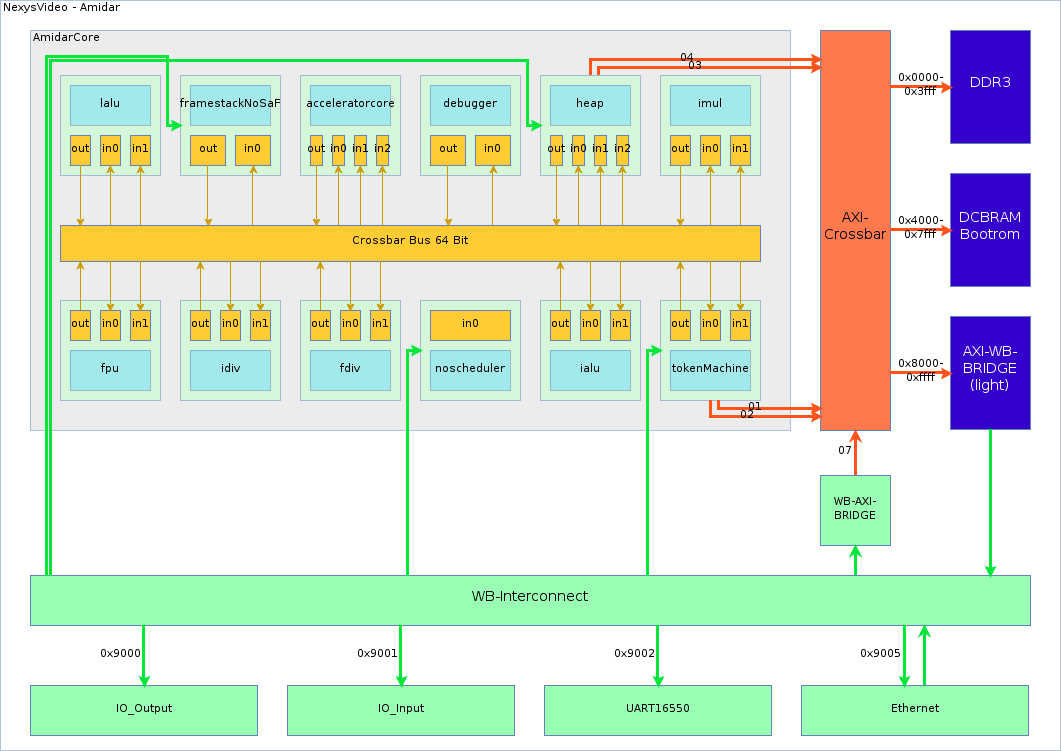
\includegraphics[width = 1\textwidth]{Graphics/system.png}
	\caption{Konfiguration des verwendeten AMIDAR-Systems, automatisch generiert durch den AMIDAR-Systembuilder}

\end{figure}

\FloatBarrier
\section{Grundlegende Funktionen}

Für das Testen der Grundfunktionen wurden mehrere Testszenarien verwendet. Zum einen wurde ein einfacher Echo-Server auf AMIDAR laufen gelassen, der ankommende Wörter zurücksendet. Dieser wurde auf einem oder mehreren Threads aufgeführt. Eine auf dem Laptop laufende Java-Anwendung sendet dabei eingegebene Textnachrichten und wartet auf die Antwort des Servers, welche in der Konsole ausgegeben wird. Dabei wird sowohl der Verbindungsaufbau als auch das Empfangen und Senden von Nachrichten getestet. Dies funktioniert auch mit mehreren offenen Verbindungen parallel. \\\\
Eine Anfrage bei einem DHCP Server funktioniert ebenfalls problemlos, wie sich dem Wireshark Screenshot im Anhang entnehmen lässt. \autoref{DHCP}




\section{Leistung}
Für die Leistungsmessung wird eine Mischung von Daten verwendet, die entweder mit Wireshark ausgelesen wurden, in den Testanwendungen auf dem Laptop in eine .csv Datei geloggt, oder während dem Betrieb auf AMIDAR ermittelt und über UART ausgegeben wurden. 
Die Latenz der einzelnen Pakete wurde Wireshark entnommen. Da Wireshark auf dem Laptop lief, ist die Übertragungszeit des letzten Pakets, das vom Laptop in einem Handshake gesendet wurde nicht gemessen worden. \\
Beim drei Wege Handshake, der von dem Laptop initiiert wurde, betrug die RTT nach dem Senden des SYN-Paketes bis zum Eintreffen des SYN-ACK-Pakets 15-30 Millisekunden. Momentan gibt es eine recht große Schwankung der Reaktionszeit. 

Falls die Übertragung von AMIDAR initiiert wird, benötigt der Laptop 900 Millisekunden, um auf die Anfrage zu reagieren. Nach weiteren 40 Millisekunden trifft das ACK-Paket von AMIDAR ein.\\\\
In einem weiteren Test wurden zehn Verbindungen zum selben Zeitpunkt geöffnet, über die jeweils in kurzen Abständen 500 Byte an Daten übertragen wurden. Diese Daten wurden von AMIDAR als Echo zurückgesendet. Dieses Szenario soll einen Server-Betrieb simulieren, bei dem Anfragen mehrerer Clients beantwortet werden sollen. Die Latenz dieser Übertragung wurde in einer Logdatei gespeichert und betrug zwischen 1,4 und 3,5 Sekunden. Dabei entfiel der größte Teil der Zeit auf das Auslesen der Daten aus den ankommenden Datenpaketen.\autoref{Multithread}\\

\begin{tabular}{cccc}
\# & Start Time$[ms]$ & End Time $[ms]$ & Response Time$[ms]$\\
1 &1495793145037&	1495793148691&	3654\\
2 &1495793149191&	1495793151370&	2179\\
3 &1495793151871&	1495793153906&	2035\\
4 &1495793154406&	1495793156688&	2282\\
5 &1495793157188&	1495793158886&	1698\\
6 &1495793159387&	1495793160988&	1601\\
7 &1495793161489&	1495793163013&	1524\\
8 &1495793163513&	1495793164989&	1476\\
\end{tabular}\\\\
Auffällig dabei ist, dass die Reaktionszeiten der einzelnen Verbindung mit weiteren Iterationen besser werden. \\
Bei diesem Testszenario wurden mit dem Statistik-Modul der AMIDAR-IDE folgende Werte ermittelt:\\\\
\begin{tabular}{lc}
jumpBytecodes & 16842753\\
total & 545259268 \\
distributedToken & 2004025412 \\
axi.transaction& 1\\
cache.hit & 65793\\
cache.hitrate& 0.996109\\
cache.miss& 257\\
outputFifoEmptyAtferFirstTransaction&16780707
\end{tabular}\\\\
Ein Problem, das bei diesem Versuch sichtbar wurde, ist die schwankende Latenz. Die Dauer eines Timeouts wird bei TCP relativ zur RTT bestimmt. Nach dem schnellen SYN-ACK mit kleinen Paketen wird im PC ein entsprechend kurzes Zeitlimit für Timeouts gesetzt. Das hat zur Folge, dass es zu Neuübertragungen größerer Datenpakete kommen kann, wenn diese auf der Seite des AMIDAR-Prozessors verarbeitet werden müssen, obwohl sie nicht verloren gegangen sind. \autoref{ret} \\\\
Die Übertragungsrate beim Senden wurde ermittelt, in dem ein zufällig generiertes Datenpaket in einer Schleife gesendet wurde. Dabei wird eine Übertragungsrate von 1333 kBit/s erreicht. Die Größe der einzelnen Datenpakete hat dabei nur einen vernachlässigbaren Einfluss auf die Nettoübertragungsrate, was darauf schließen lässt, dass das Bottleneck bei dem Sendepuffer liegt. \\\\
Dabei wurden mit dem Statistik-Modul des Debuggers folgende Werte ermittelt:\\\\
\begin{tabular}{lc}
jumpBytecodes & 537919489\\
total & 545259268 \\
distributedToken & 393412689 \\
axi.transaction& 1\\
cache.hit & 65793\\
cache.hitrate& 0.9960939\\
cache.miss& 258\\
outputFifoEmptyAtferFirstTransaction & 16781085
\end{tabular}






 

 
\chapter{Zusammenfassung}


\section{Fazit}

\section{Ausblick}

\begin{appendix}
  
\chapter{Anhang}

\subsection{Senden von Daten über eine Verbindung}



\section{Wireshark Screenshots}
\begin{figure}
	\centering
	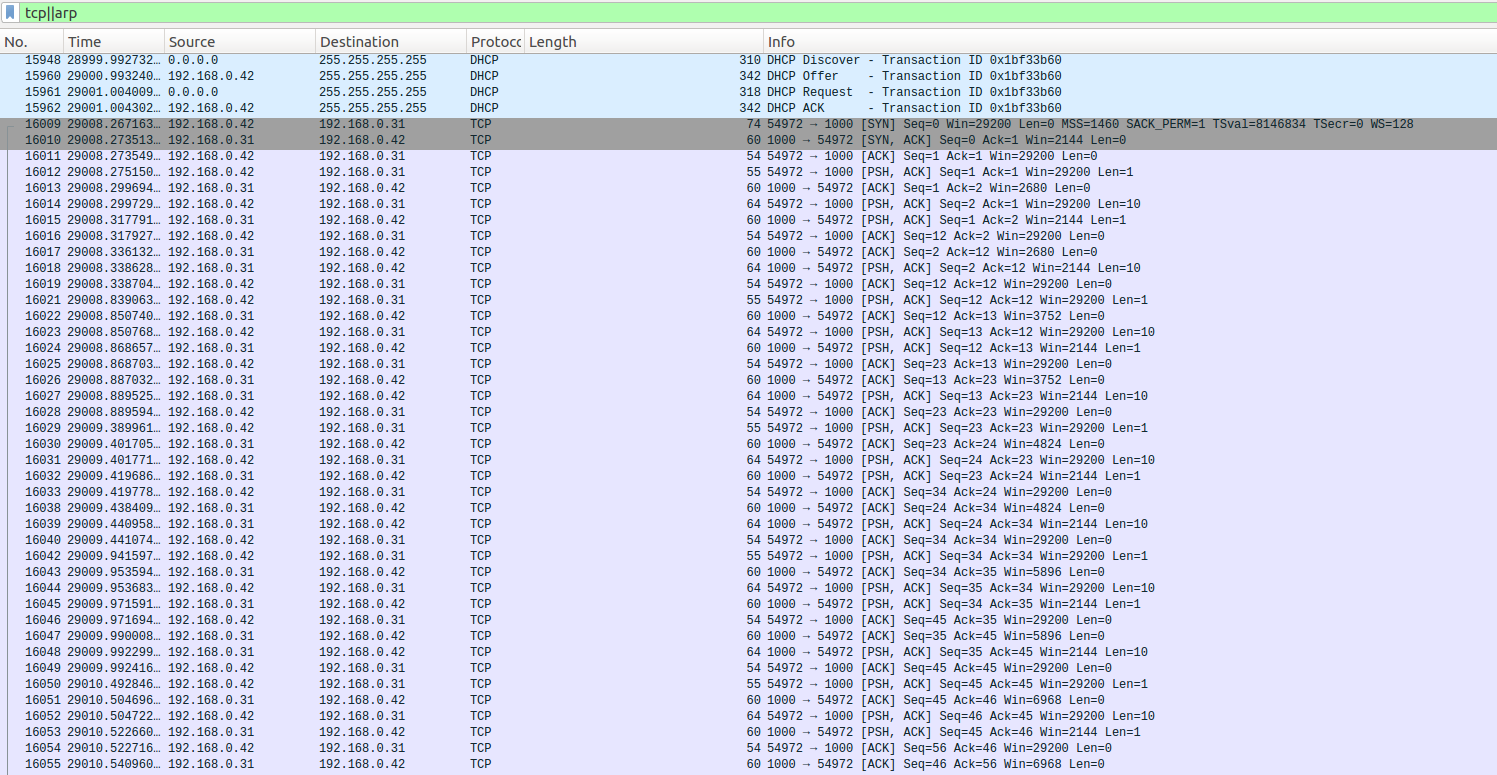
\includegraphics[width=1\textwidth]{Graphics/dhcpHD.png}
	\caption{DHCP, Drei-Wege-Handschlag, Datenübertragung}
	\label{DHCP}
	
\end{figure}

\begin{figure}[h]
	\centering
	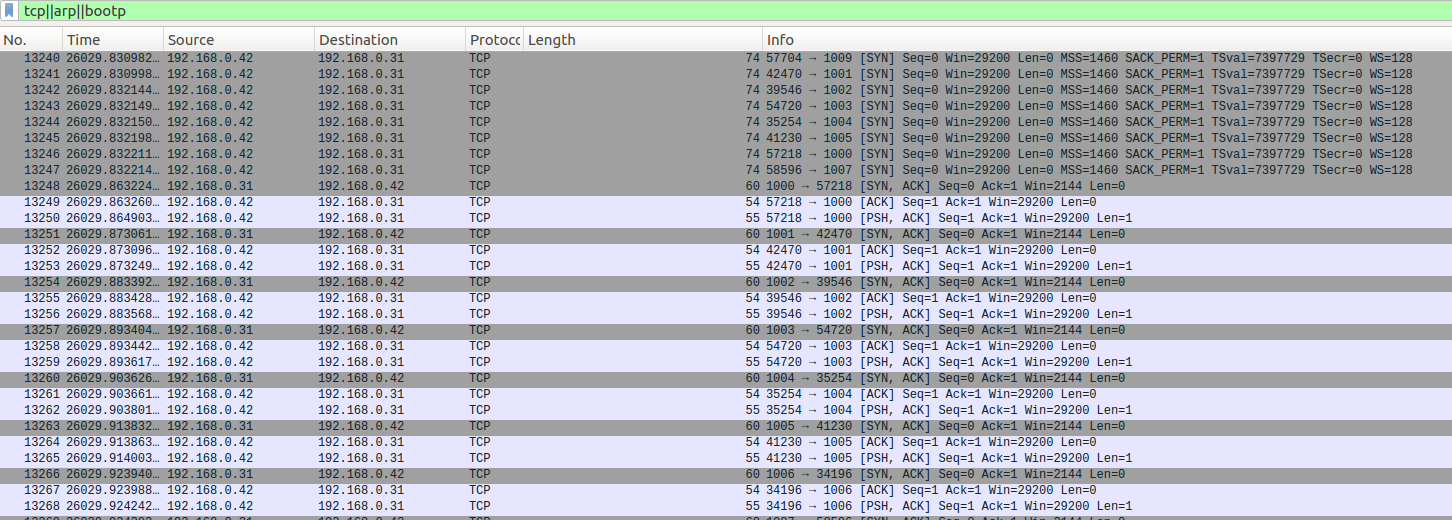
\includegraphics[width=1\textwidth]{Graphics/MTCon.png}
	\caption{Gleichzeitiger Verbindungsaufbau mehrerer Verbindungen}
	\label{Multithread}
\end{figure}

\begin{figure}[h]
	\centering
	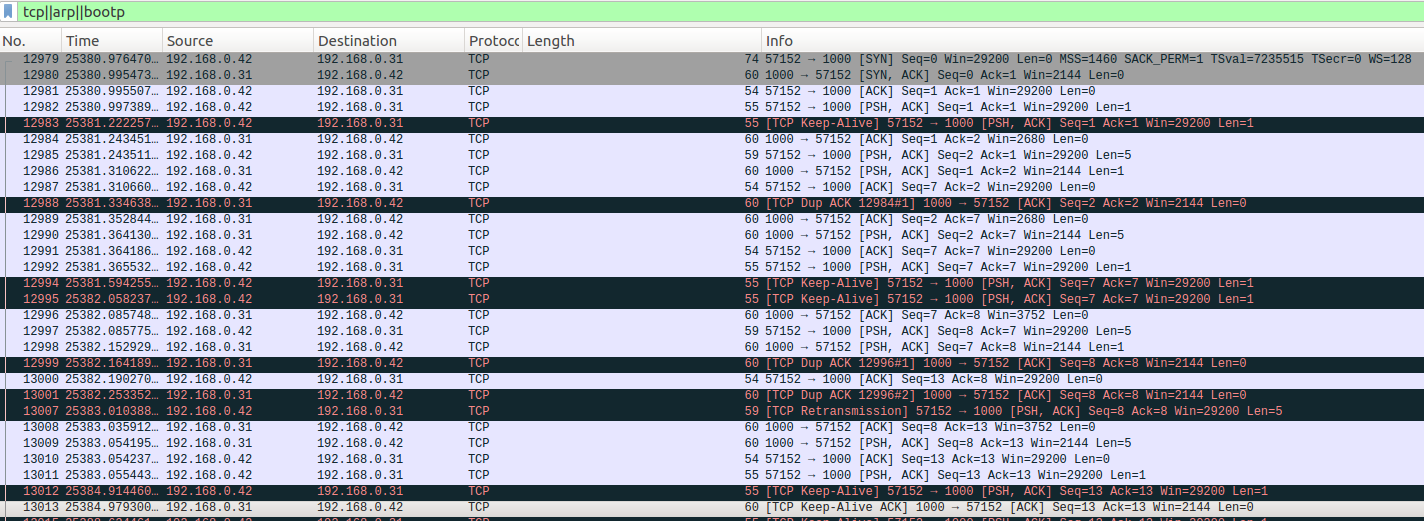
\includegraphics[width=1\textwidth]{Graphics/latency.png}
	\caption{keep-alive und Retransmissions, wegen schwankender Latenz, bei großen Datenpaketen}
	\label{ret}
\end{figure}
\end{appendix}

\cleardoublepage

\section*{Abkürzungsverzeichnis}
\begin{acronym}

 \acro{CPU}{central processing unit}
 \acro{FPGA}{Field Programmable Gate Array} 
 \acro{RTT}{Round Trip Time}
\acro{AMIDAR} {Adaptive Microinstruction Driven ARchitecture}
\acro{IP}{Internet Protocol}
\acro{TCP}{Transmission Control Protocol}
\acro{UDP}{User Datagram Protocol}
\acro{API}{Application Programming Interface}
\acro{MAC}{Media-Access-Control}
\acro{IEEE}{Institute of Electrical and Electronics Engineers}
\acro{TTL}{Time to Live}
\acro{FU}{Function Unit}
\acro{ALU}{arithmetic logic unit}

\end{acronym}


\listoffigures
\cleardoublepage

\makeatletter

\renewcommand\chapter{\thispagestyle{\chapterpagestyle}%
                    \global\@topnum\z@
                    \@afterindentfalse
                    \secdef\@chapter\@schapter}
\makeatother

\nocite{*}
\bibliographystyle{alphadin}
\bibliography{Literaturverzeichnis}



\end{document}